\chapter{Résultats des benchmarks}

Nous allons maintenant présenter les résultats obtenus suite à l'exécution des scripts de benchmarking.

Tout d'abord, nous présenterons les métriques retenues pour chaque benchmark. Puis, nous analyserons les données, qui seront visualisables sous forme de graphes, afin de permettre de résoudre le problème de la partie suivante.

\section{Choix des métriques}
\paragraph{CPU} Avec \textit{Sysbench}, nous avons choisi de conserver le résultat du temps total d'exécution, ainsi que le temps moyen d'exécution par requête. Ce sont les deux métriques les plus représentatives des performances du CPU d'une instance.

%% ça serait peut-être mieux de prendre plutôt le '95 percentile' plutôt que la moyenne car au final temps total et moyenne disent la même chose...

\paragraph{IO} Pour \textit{dd}, nous avons choisi le débit d'entrées/sorties car c'est le seul résultat qui a un rapport avec la performance du système en matière d'IO. En effet, il serait inutile de choisir le temps d'exécution car il ne donne aucune information (combien de données ont été copiées pendant ce temps ? qu'est-ce que cette valeur représente vraiment ?).

\paragraph{IOPS} Pour \textit{Bonnie++}, intéressons-nous d'abord aux résultats de sortie du test. Les différentes informations signifient :
\begin{itemize}
  \item \%CPU : pourcentage du CPU utilisé pour le test
  \item create, read, delete : création, lecture puis suppression de fichiers de zéro octet
  \item Sequential Create : les opérations sont réalisées sur des fichiers avec un nom trié numériquement (accès séquentiel)
  \item Random Create : les opérations sont réalisées sur des fichiers avec un nom aléatoire (accès aléatoire)
  \item Sequential Input : lectures séquentielles
  \item Sequential Output : écritures séquentielles
  \item Random Seeks : nombre de recherches aléatoires par seconde
  \item +++++ : opération trop rapide pour être mesurée
\end{itemize}

Nous avons choisi de conserver les métriques \textit{Sequential output per char}, \textit{Sequential input per char}, et \textit{Random seeks}, ainsi que la latence respective pour chacune de ces opérations. Il est important de conserver la latence car elle peut varier selon le type de disque (HDD ou SSD par exemple). 

Nous ne gardons pas les informations par bloc car nous avons déjà celles par caractère. Comme les opérations de \textit{create, read, delete} donnent des résultats trop rapides pour la plupart des instances, nous n'exploitons pas ce résultat (nous ne pouvons pas faire de comparaison alors qu'il manque des données). Nous ne conservons pas non plus les données concernant le pourcentage d'utilisation du CPU, car ce n'est pas ce qui nous intéresse ici (nous voulons des informations sur les IOPS).

\paragraph{Mémoire}

A la sortie du benchmark \textit{Stress-ng}, plusieurs métriques sont disponibles : 
\begin{itemize}
  \item bogo ops : nombre d'itérations du stresseur effectuées
  \item real time : durée 'wall clock' (moyenne) du stresseur (s)
  \item usr time : durée utilisateur totale (s)
  \item sys time : durée système totale (s)
  \item bogo ops/s (real time) : "total bogo operations per second based on wall clock run time. The wall clock time reflects the apparent run time. The more processors one has on a system the more the work load can be distributed onto these and hence the wall clock time will reduce and the bogo ops rate will increase. This is essentially the "apparent" bogo ops rate of the system."
  \item bogo ops/s (usr+sys time) : "total bogo operations per second based on cumulative user and system time. This is the real bogo ops rate of the system taking into consideration the actual time execution time of the stressor across all the processors. Generally this will decrease as one adds more concurrent stressors due to contention on cache, memory, execution units, buses and I/O devices."
\end{itemize}

L’outil nous propose donc plusieurs métriques après le test, et nous avons opté pour le bogo ops/s (usr+sys time) parce qu’il nous donne le taux réel de \textit{bogo operations} du système en tenant compte du temps d’exécution réel du facteur de stress sur tous les processeurs, comme cela a été souligné précédemment. 

\paragraph{Disque}

Pour \textit{hdparm}, l’outil nous donne les valeurs de cached reads et buffered disk. Pour nous qui cherchons à connaître la vitesse de lecture, utiliser ces deux métriques nous est plus logique et plus bénéfique car elles nous permettent d'obtenir les valeurs de vitesse de lecture en détail.

\paragraph{Réseau}

Pour \textit{speedtest}, nous avons les résultats comme pour tout test de vitesse du réseau, les 2 éléments importants pour le débit, c’est-à-dire le débit descendant (download) et le débit montant (upload). Donc cet outil donne exactement les deux métriques qu’il faut pour mesurer les performances réseau de nos instances.

\section{Analyse des résultats}

Nous allons maintenant étudier les résultats obtenus avec nos benchmarks. Chaque valeur correspond à la moyenne des 5 valeurs (chacune ayant été obtenue dans une itération du benchmark).

Un tableau récapitulant toutes les données est disponible en annexe (\ref{tab_recap}).

\paragraph{CPU}

Comme nous pouvons le voir avec la figure \ref{fig:cpu}, l'instance présentant les meilleures performances pour le CPU est Amazon C4, avec une moyenne de 2.5ms de temps d'exécution par requête. En comparaison, la machine la moins performante est Azure A1 avec 6.69ms en moyenne par requête, soit plus du double du temps affiché par Amazon C4. 

Ces résultats étaient prévisibles, puisque Azure A1 ne possède qu'un seul coeur alors que Amazon C4 en a 16 (avec un CPU bien plus rapide). Toutefois, il faut noter que les performances de l'instance Azure A4 ne correspondent pas à ce à quoi on aurait pu s'attendre. En effet, ses performances (6.66ms/requête) sont proches de celles de Azure A1, alors qu'elle a 4 coeurs et un meilleur CPU. Même la moins bonne machine Amazon (Amazon T2) qui ne possède qu'un coeur est plus performante, ce qui s'explique peut-être par un modèle de CPU supérieur.

\begin{figure}[h]
  \begin{center}
    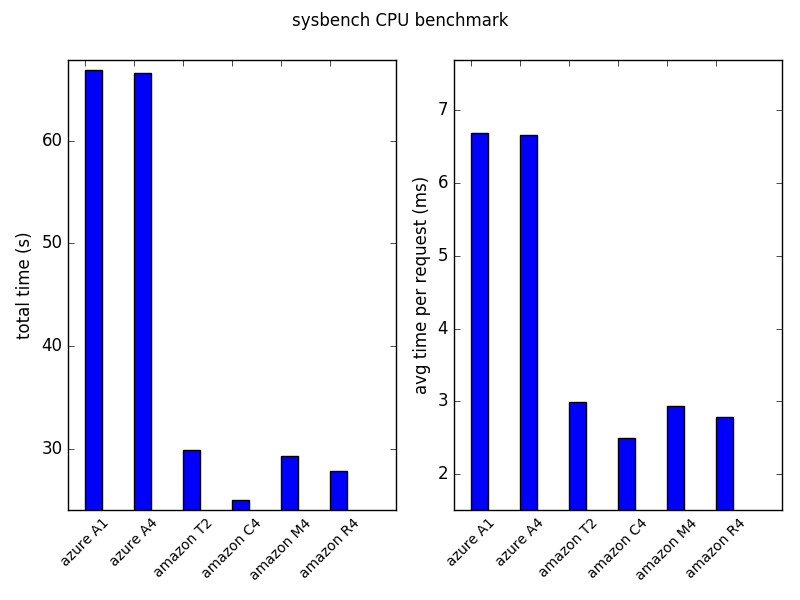
\includegraphics[width=\textwidth]{plot_CPU.png}
    \caption{Résultats du benchmark Sysbench pour chaque instance}
    \label{fig:cpu}
  \end{center}
\end{figure}

\paragraph{IO}

Nous nous intéressons à présent au débit d'entrée/sortie. L'instance Amazon C4 a les meilleures performances, avec 145 MB/s, suivie de Amazon M4, avec 131 MB/s. La moins bonne machine est Azure A4 avec 33.5 MB/s, ce qui est bien inférieur au débit des autres machines. La meilleure machine a donc un débit un peu plus de 4 fois supérieur à celui de la moins bonne machine, ce qui constitue un écart important à prendre en compte lors du choix des instances.

Les résultats peuvent être visualisés avec la figure \ref{fig:io}.

Avec leur disque SSD, il est cohérent de constater que les machines Amazon ont de meilleures performances que les machines Azure.

\begin{figure}[h]
  \begin{center}
    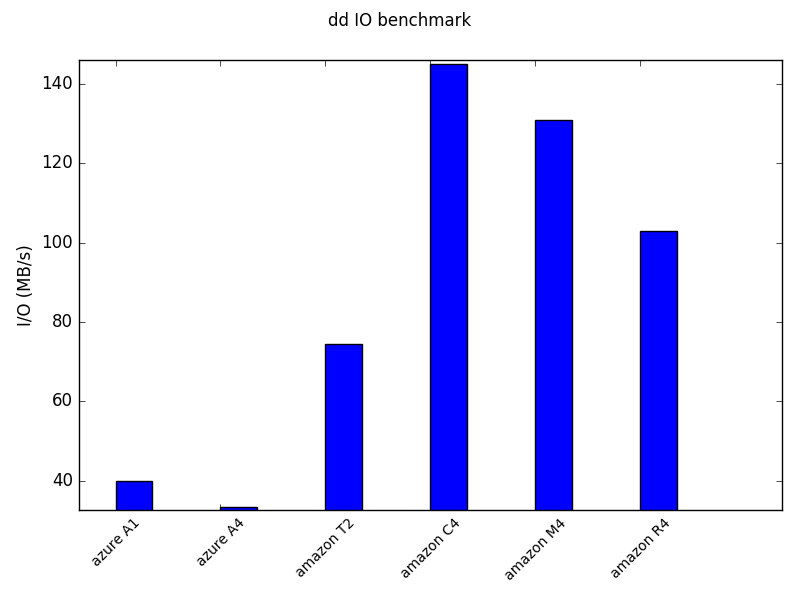
\includegraphics[width=\textwidth]{plot_IO.png}
    \caption{Résultats du benchmark dd pour chaque instance}
    \label{fig:io}
  \end{center}
\end{figure}

\paragraph{IOPS}

Pour les lectures et écritures séquentielles, c'est Amazon C4 qui a encore une fois les meilleures performances, avec le plus grand débit, comme on peut le voir sur la figure \ref{fig:iops} (1296.2K/s en écriture et 5900.6K/s en lecture). De manière générale, les 3 autres instances Amazon présentent des performances assez similaires, et supérieures aux performances des instances Azure. Il est intéressant de remarquer que l'instance Amazon T2 a de meilleures performances en écriture (1201.2K/s) que les instances M4 et R4 (resp. 1088.8K/s et 1119.8K/s), alors qu'en lecture, ses performances (4872.2K/s) sont un peu moins bonnes que ces dernières (resp. 4998.4K/s et 4888.2K/s).

Pour les recherches aléatoires, il manque des données pour les instances Amazon R4, C4 et M4 car les opérations ont été trop rapides.

Dans tous les cas, l'instance avec la plus petite latence est Amazon C4 (qui est très faible pour les recherches aléatoires, avec seulement 34us de latence contre 319.4us pour la deuxième meilleure machine et 203000us pour la moins bonne). Les deux machines Azure sont celles avec la plus grande latence, en particulier l'instance A1 qui a une latence bien plus élevée que la A4 pour les lectures séquentielles (resp. 33882us contre 10888us) et les recherches aléatoires (resp. 203000us contre 19529us).

\begin{figure}[h]
  \begin{center}
    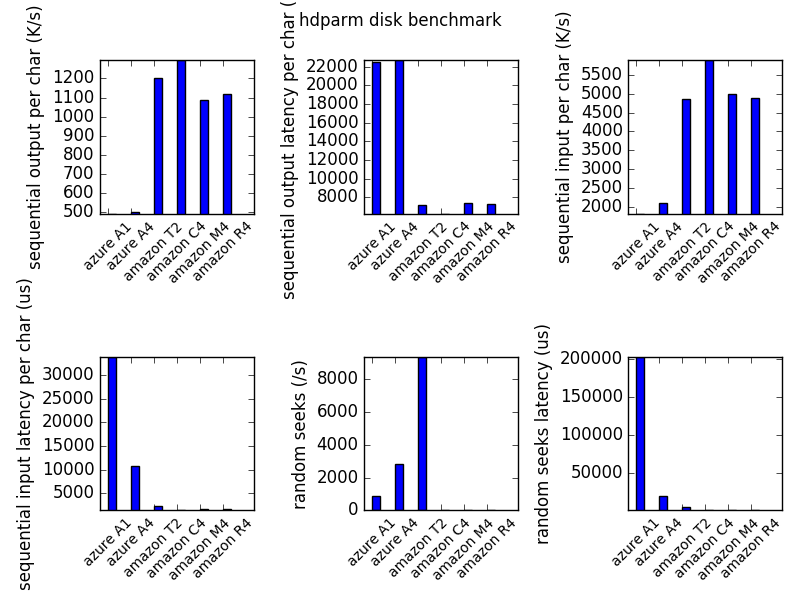
\includegraphics[width=\textwidth]{plot_IOPS.png}
    \caption{Résultats du benchmark Bonnie++ pour chaque instance}
    \label{fig:iops}
  \end{center}
\end{figure}

\paragraph{Mémoire}

\begin{figure}[h]
  \begin{center}
    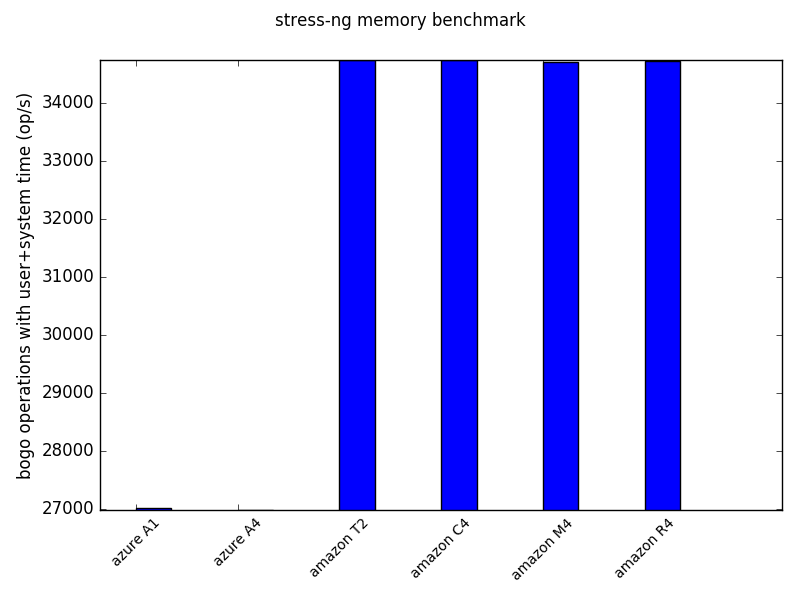
\includegraphics[width=\textwidth]{plot_memory.png}
    \caption{Résultats du benchmark stress-ng pour chaque instance}
    \label{fig:memoire}
  \end{center}
\end{figure}

Pour ce qui est du test de la mémoire, il s’agit de tester la stabilité du système lorsque la charge est élevée, autrement dit s’il est soumis à un fort stress. Comme on peut le voir sur la figure \ref{fig:memoire}, les instances Amazon sont les plus performantes avec une moyenne de 34500 bogo ops/s. Nous avons également constaté une différence assez grande par rapport aux instances Azure qui ont 27000 bogo ops/s en moyenne. En comparant de plus près une instance Amazon (r4) et une Azur (A4m2) ayant des caractéristiques presque similaires, la différence de performance est quand même étonnante. 

\paragraph{Disque}

\begin{figure}[h]
  \begin{center}
    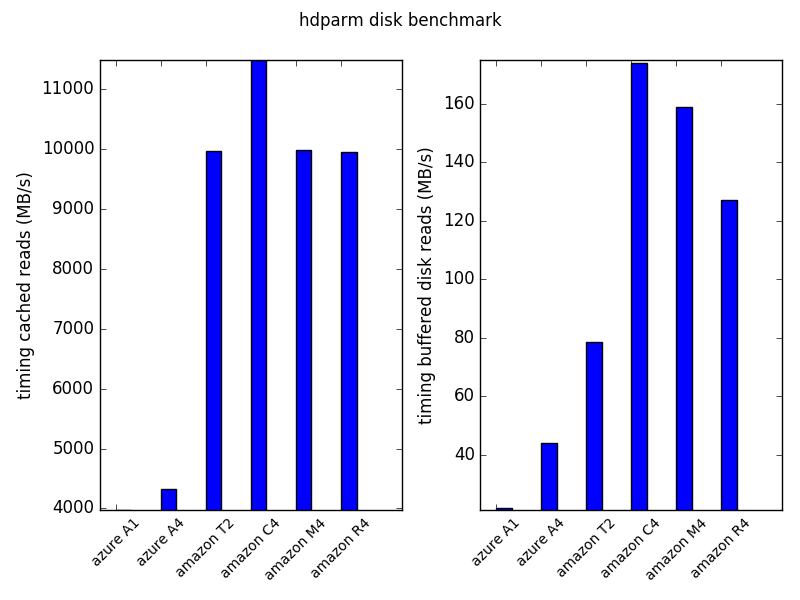
\includegraphics[width=\textwidth]{plot_disk.png}
    \caption{Résultats du benchmark hdparm pour chaque instance}
    \label{fig:disque}
  \end{center}
\end{figure}

Ici, l’objectif est de tester la vitesse de lecture (buffered read et cached read) et comme nous pouvons le constater sur la figure \ref{fig:disque}, les instances Amazon sont les plus performantes sur le point de vue vitesse de lecture, avec en tête l’instance C4 (11489MB/s de timing disk reads et 173.898MB/s de timing buffered disk reads) et la moins performante est la machine A1 d’Azure (3966.54MB/s de timing disk reads  et 21.96MB/s de timing buffered disk reads)

\paragraph{Réseau}

\begin{figure}[h]
  \begin{center}
    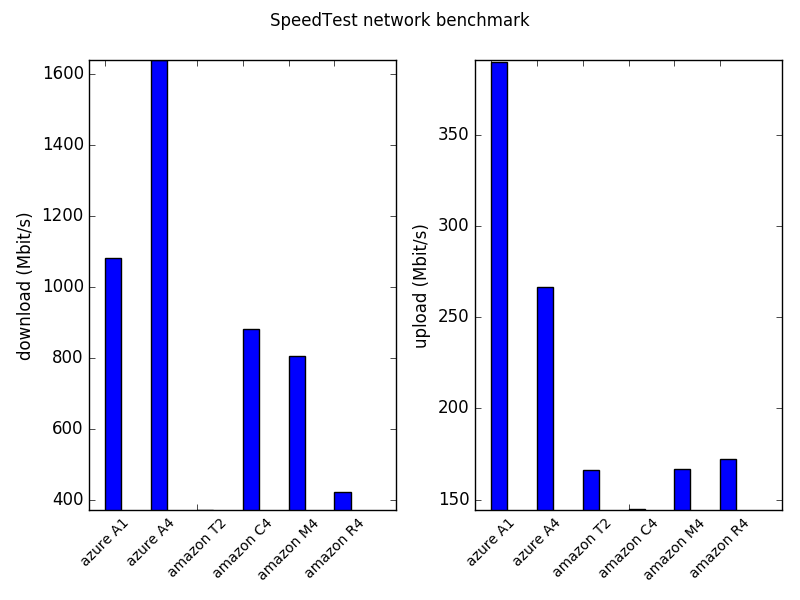
\includegraphics[width=\textwidth]{plot_network.png}
    \caption{Résultats du benchmark Speedtest pour chaque instance}
    \label{fig:reseau}
  \end{center}
\end{figure}

Sur ce point, il était question de tester les débits de Download et Upload de nos instances de ces différents fournisseurs (Amazon et Azure). Les résultats de ces tests nous montrent que les instances Azure sont les plus performantes en terme de vitesse, avec en tête l’instance A4m2 qui a 1638.51Mbit/s de débit download et 266.74Mbit/s en upload, et que celle d’Amazon qui la plus performante est C4 avec 881.72Mbit/s de download et 145Mbit/s d’upload.
Nous remarquons que parmi les deux instances d’Azure, la A4m2 (1638.51MB/s) a une vitesse download supérieure à la A1 mais en upload c’est l’instance A1 qui a une valeur supérieure et c’est pareil pour les autres instances. Donc, l’instance qui a une grande vitesse de Download n’est pas nécessairement celle qui a la plus grande valeur en Upload.


\section{Remarques} 

De manière générale, la grande différence de performances entre les instances Azure et celles Amazon est étonnante. Toutefois, nous avons effectué les benchmarks à plusieurs reprises et nous avons obtenus des résultats similaires. Nous n'avons pas d'explication concernant un tel phénomène car même pour des caractéristiques similaires, les instances Amazon ont des performances bien meilleures que celles Azure.